
\chapter{位置制御}位置制御とは,制御対象の現在位置を何らかのセンサなどで検出し,目標の位置になるようにフィードバック制御を行うことである.

\section{位置検出}今回のリフトのようにモータを動力とする位置制御をする際は,ロータリーエンコーダでモータの回転角度を検出し,ギヤ比やスプロケット半径から計算して制御対象の位置を特定する.このように,位置制御を行う際は位置を直接取得できるセンサを使用して,その値をフィードバックするのが一般的である.

\section{制御手法}
制御には主に以下のような手法が使われる.

\subsection{PID制御}目標値と現在値の差のことを偏差という.偏差に比例して制御量が増える制御を比例制御(P)といい,比例定数Kpは比例ゲインと呼ばれる.比例制御では偏差が0になると制御量が0になるため,いつまでたっても偏差が残り続ける事がある.この残留偏差をなくすため,偏差を時間で積分したものをKi倍して制御量に加えると,残留偏差のある時間が長いほど制御量が増えていき最終的に偏差が無くなる.これを積分制御(I)といい,Kiは積分ゲインと呼ばれる.偏差が急激な変化をする動き始めと動き終わりには,偏差を微分した値が大きくなる.微分に比例して制御量を大きくすると機敏な動作をするようになり,早く目標値に到達する.これを微分制御(D)といい,この比例定数Kdは微分ゲインと呼ばれる.これらP,I,D制御を組み合わせた基本的な制御手法がPID制御(図\ref{fig:PID})である.

\begin{figure}[htbp]
  \begin{center}
    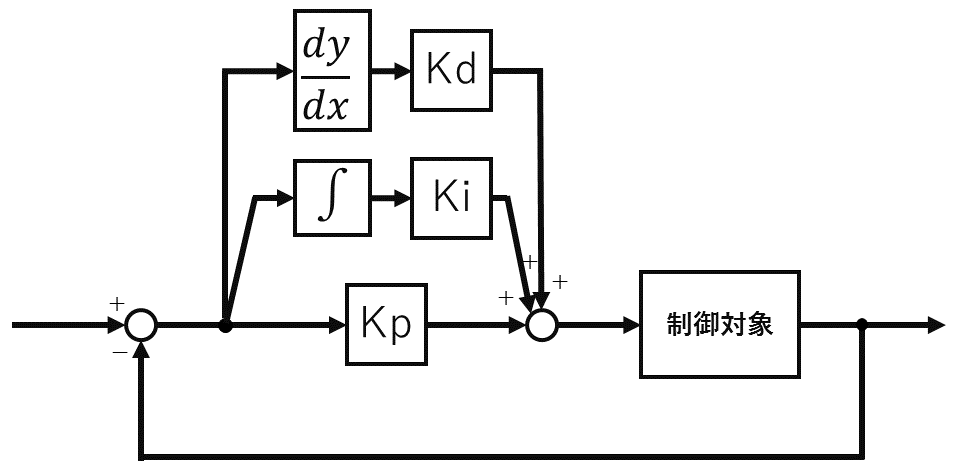
\includegraphics[width=135mm]{img/PID.png}
    \end{center}
  \caption{PID制御のブロック線図}
 \label{fig:PID}
\end{figure}

\subsection{極配置法}システムは式(\ref{eq:joutai})のような状態方程式という形で表すことが出来る.状態方程式はシステムへの入力$u$,システムからの出力$y$,システムの状態量$x$の関係を表した方程式である.システムは極と呼ばれる固有の値を持っており,その値によって応答速度や行き過ぎ量などの特性が変化する.状態方程式で表されたシステムに対し,状態量$x$に一定の値(ゲイン)を掛けて入力にフィードバックすることで極を変化させることができる.極を望ましい値に設定するフィードバックゲインを探る方法を極配置法という.

\begin{eqnarray}
\begin{array}{l}
\dot{x}=\bm{A}x+\bm{B}u\\
y=\bm{C}x+\bm{D}u
\end{array}
\label{eq:joutai}
\end{eqnarray}
